% !TeX root = ../notes.tex

\chapter{Exploring chemical space}

\begin{notebox}
  \keypoint{What do you need to learn from this chapter?}
  This chapter examines how molecular structure can be represented using numerical descriptors and how collections of molecules can be compared within multidimensional chemical spaces.
  You should understand that descriptor choice determines which molecular differences are represented, how similarity and distance depend on that representation, and why dimensionality reduction is required to visualise high-dimensional data.
  Particular emphasis is placed on connecting classical physical-organic parameters with modern molecular descriptors and on interpreting chemical-space maps critically.
\end{notebox}

\section{From physical-organic parameters to molecular descriptors}

The previous chapter used numerical parameters to describe how changes in molecular structure influence chemical behaviour.
Hammett substituent constants encode electronic effects, while Taft-type relationships introduce an additional steric contribution.
These parameters are examples of \keypoint{molecular descriptors}: numerical quantities used to describe molecular structure or properties.
A descriptor does not reproduce the complete molecule, but selects aspects of the molecule that may be relevant to the chemical question being asked.

\solution{4.0cm}{%
  \centering
  \begin{tabular}{@{}ll@{}}
    \textbf{Hammett:} & molecule $\longrightarrow \sigma_{\mathrm{X}}$ \\[0.55em]
    \textbf{Taft:} & molecule $\longrightarrow \left(\sigma_{\mathrm{X}},E_{\mathrm{s},\mathrm{X}}\right)$ \\[0.55em]
    \textbf{Modern:} & molecule $\longrightarrow \mathbf{x}=\left(x_1,x_2,\ldots,x_p\right)$
  \end{tabular}
}

The descriptor vector $\mathbf{x}$ may contain experimental measurements, calculated molecular properties, or values derived directly from molecular structure.
Examples include molecular mass, polarity, orbital energies, atomic charges, steric dimensions, and counts of structural fragments.

\solution{10.0cm}{%
  \centering

  \begin{tikzpicture}[
      transform shape,
      term/.style={
        draw=darkBlue,
        fill=paleBlue,
        line width=2.0pt,
        minimum width=8.0cm,
        minimum height=1.0cm,
        align=center,
        font=\sffamily
      },
      arrow/.style={
        ->,
        >=Stealth,
        draw=darkGrey,
        line width=2.3pt
      }
    ]

    \node[term] (structure) at (0,3.6)
      {molecular structure};

    \node[term] (descriptors) at (0,1.8)
      {descriptor vector $\mathbf{x}=(x_1,x_2,\ldots,x_p)$};

    \node[term] (space) at (0,0)
      {a point in multidimensional chemical space};

    \draw[arrow] (structure) -- (descriptors);
    \draw[arrow] (descriptors) -- (space);

  \end{tikzpicture}
  \\[1em]
  \begin{equation}
    \mathbf{X}
    =
    \begin{bmatrix}
      x_{11} & x_{12} & \cdots & x_{1p} \\
      x_{21} & x_{22} & \cdots & x_{2p} \\
      \vdots & \vdots & \ddots & \vdots \\
      x_{n1} & x_{n2} & \cdots & x_{np}
    \end{bmatrix},
  \end{equation}
}

\begin{conceptbox}
  \keypoint{A molecular descriptor is a selective representation.}
  Descriptors make modelling possible by converting chemical structure into numerical vectors.
  Their usefulness depends on whether the encoded information is relevant to the chemical question.
  The same molecule can occupy different positions in the chemical space when described by a different set of descriptors.
\end{conceptbox}

\subsection{A modern descriptor library: kraken}

The simple descriptor vector introduced above can contain many different kinds of chemical information.
The \textit{kraken} library provides a useful example for organophosphorus ligands used in homogeneous catalysis.\mcite{Gensch2022}
Rather than describing each ligand using a single electronic or steric parameter, the library combines many calculated physicochemical descriptors, which include quantities describing electronic structure, molecular geometry, and intermolecular interactions (Fig.~\ref{fig4-1:kraken}).

\begin{figure}[h!]
    \centering
    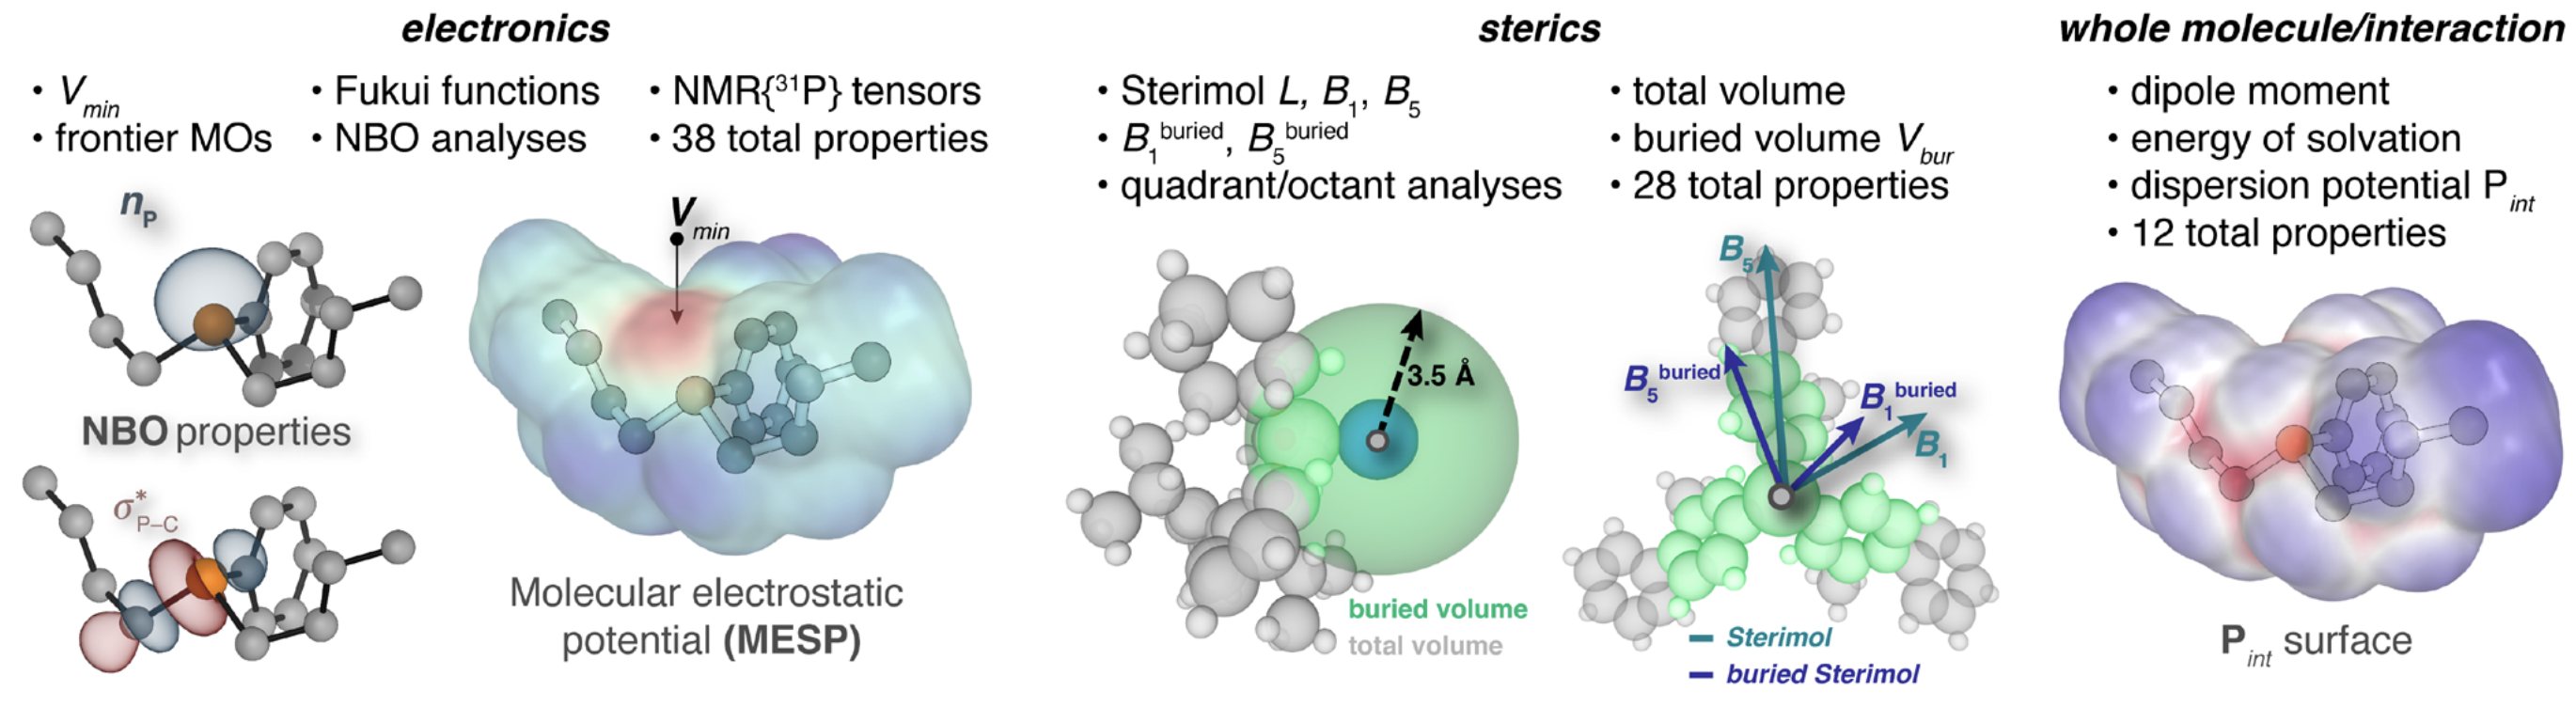
\includegraphics[width=\textwidth]{figures/CH4-kraken.png}
    \caption{Example physical organic descriptors in the \textit{kraken} library.}
    \label{fig4-1:kraken}
\end{figure}

\begin{warningbox}
Many molecular descriptors depend on three-dimensional structure.
For a flexible molecule, however, there is not one unique molecular geometry: several conformers may be accessible under the conditions of interest.
Properties can then be condensed across the ensemble in several ways, including their minimum, maximum, range, or a Boltzmann-weighted average.
\end{warningbox}

Steric effects were initially described using single numerical parameters (Fig.~\ref{fig4-2:steric-descriptor-progression}).
Examples include A-values, interference values, and the Taft steric parameter, $E_{\mathrm{s}}$.\mcite{Winstein1955,Taft1952}
These values provide useful relative measures of steric demand, but compress a three-dimensional molecular shape into one number.

\begin{figure}[htbp]
  \centering
  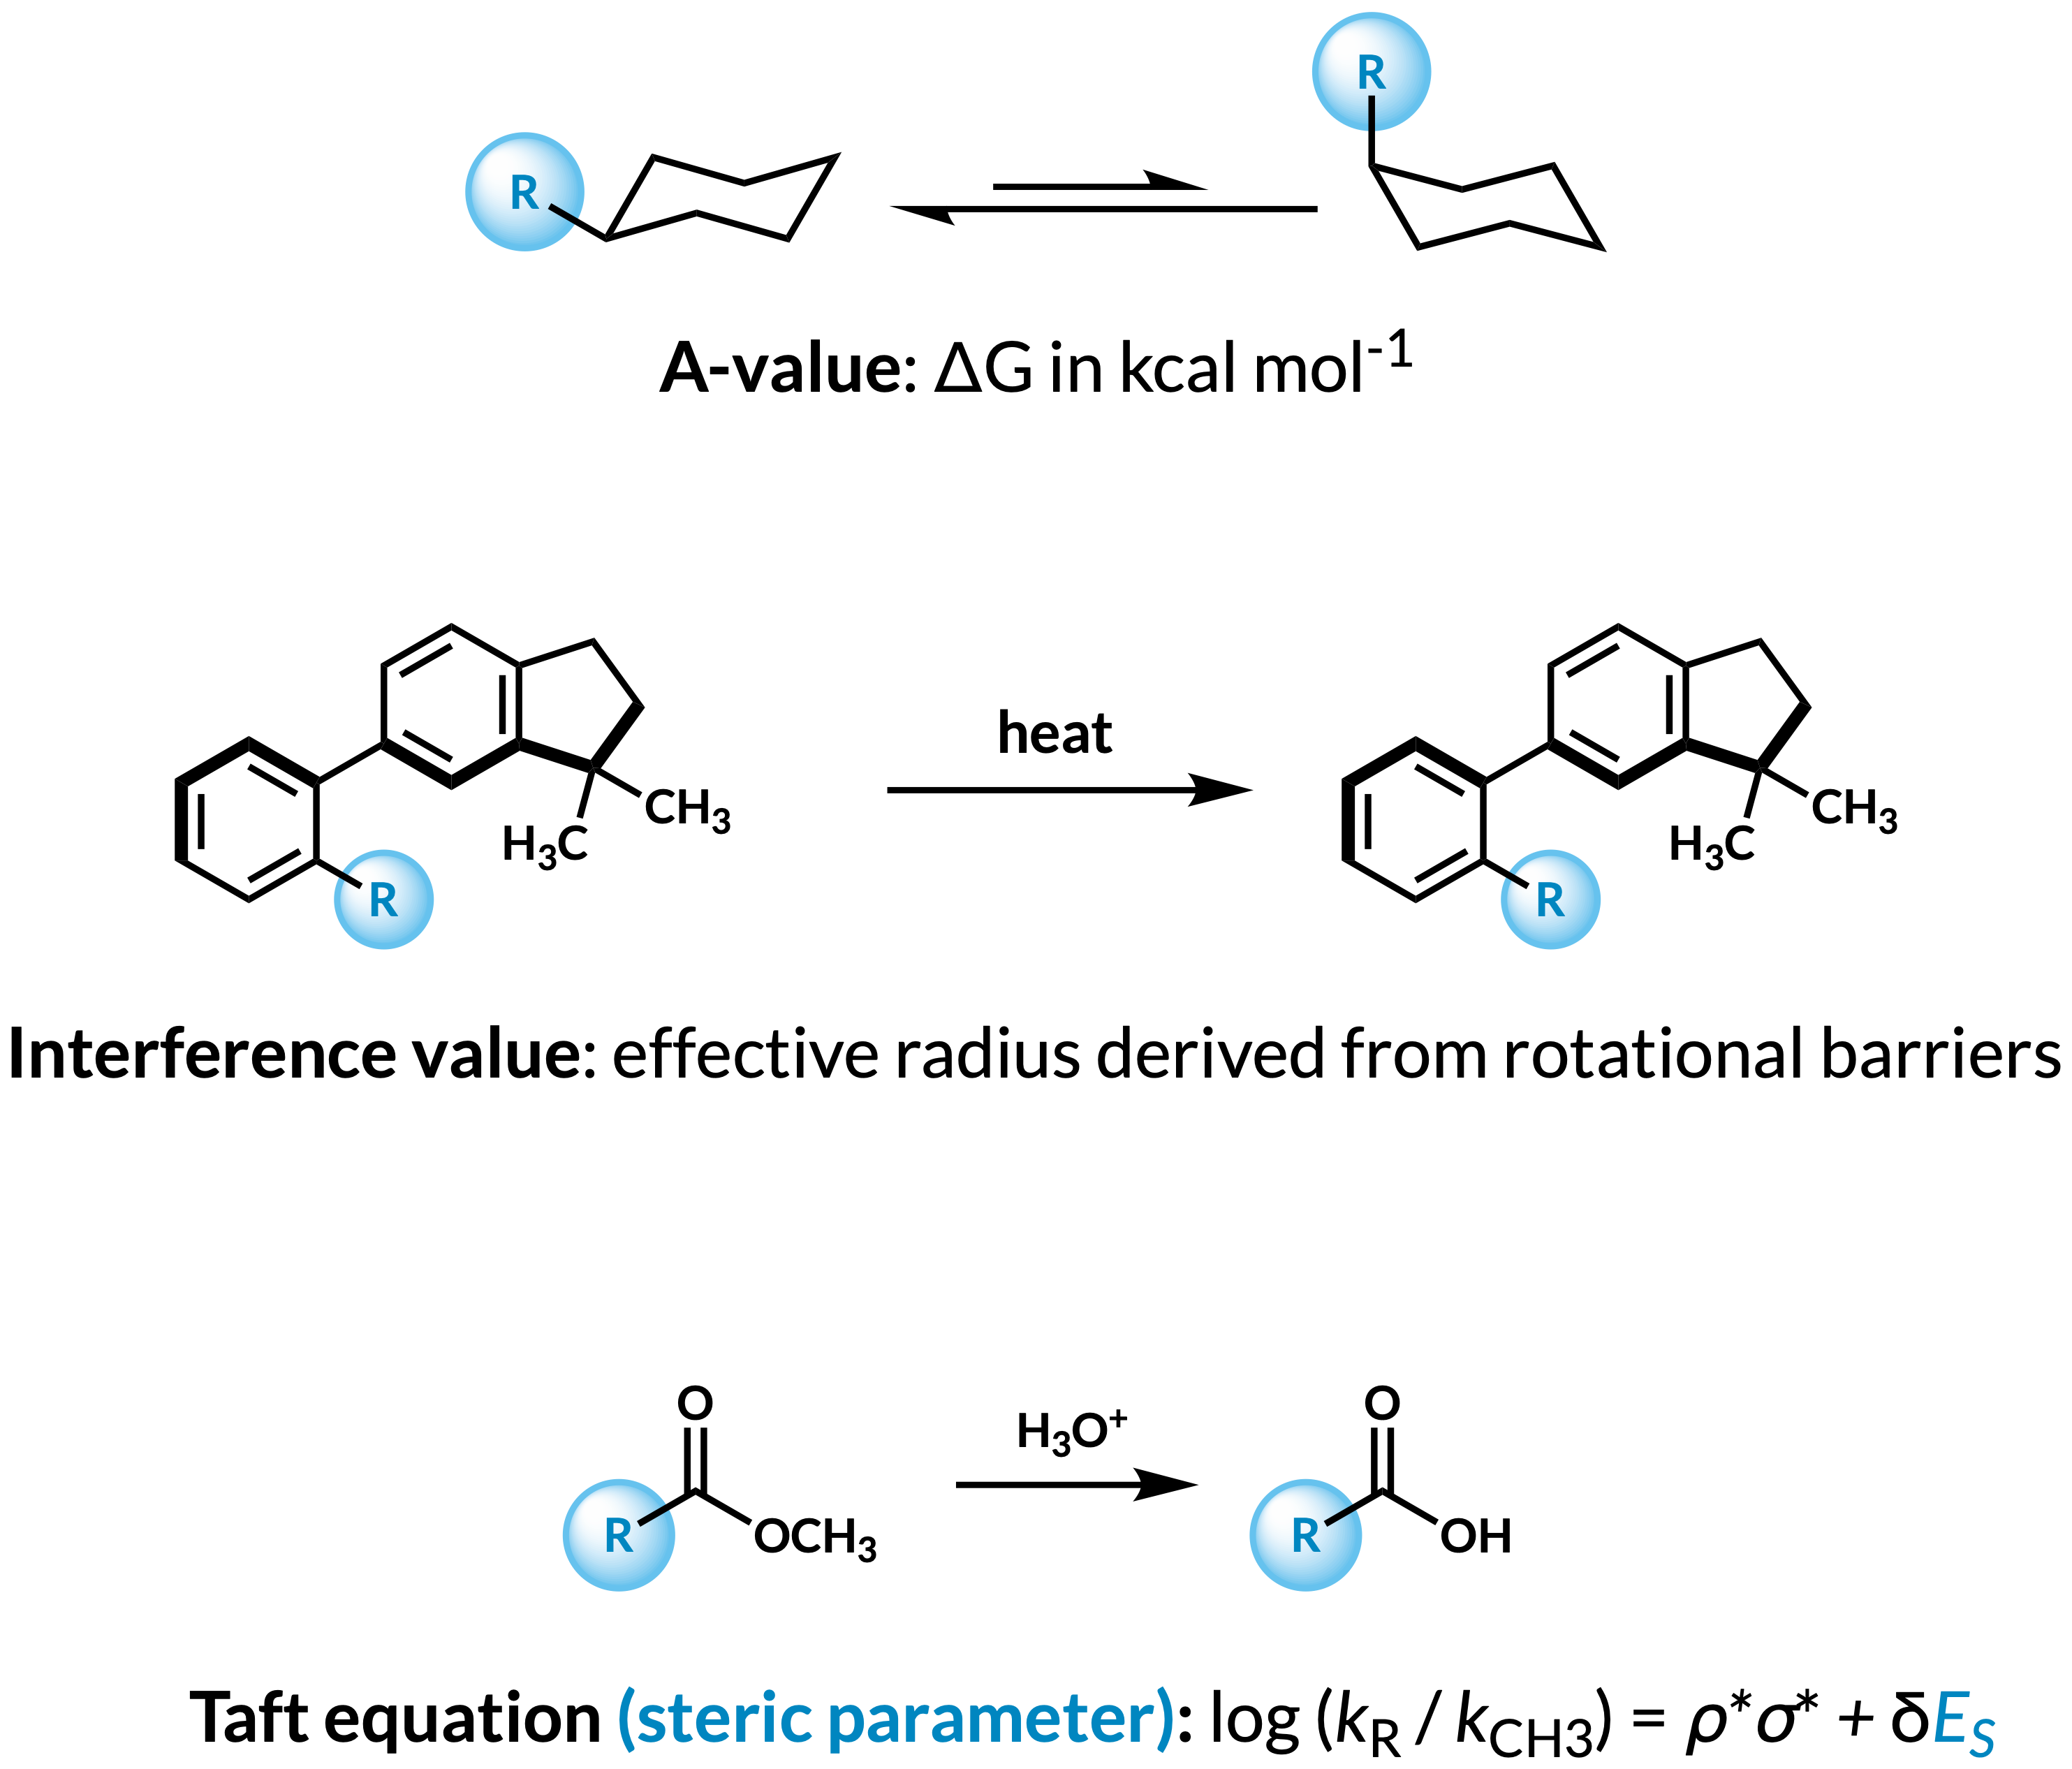
\includegraphics[width=0.75\linewidth]{figures/CH4-steric-descriptors.png}
  \caption{
    Evolution of steric descriptors from scalar parameters to directional descriptions.
    Scalar parameters such as A-values and $E_{\mathrm{s}}$ summarise steric demand using one value. 
    }
  \label{fig4-2:steric-descriptor-progression}
\end{figure}

More detailed descriptors retain information about the direction and spatial distribution of steric demand.
The Sterimol parameters are defined relative to a chosen primary axis, commonly the bond connecting a substituent to the molecular framework.\mcite{Brethome2019}
The parameter $L$ describes extension along this axis, while $B_1$ and $B_5$ describe the minimum and maximum widths perpendicular to it (Fig.~\ref{fig4-3:sterimol}).
This directional description is particularly useful for nonsymmetrical substituents that cannot be represented adequately by a single steric constant.

\begin{figure}[htbp]
  \centering
  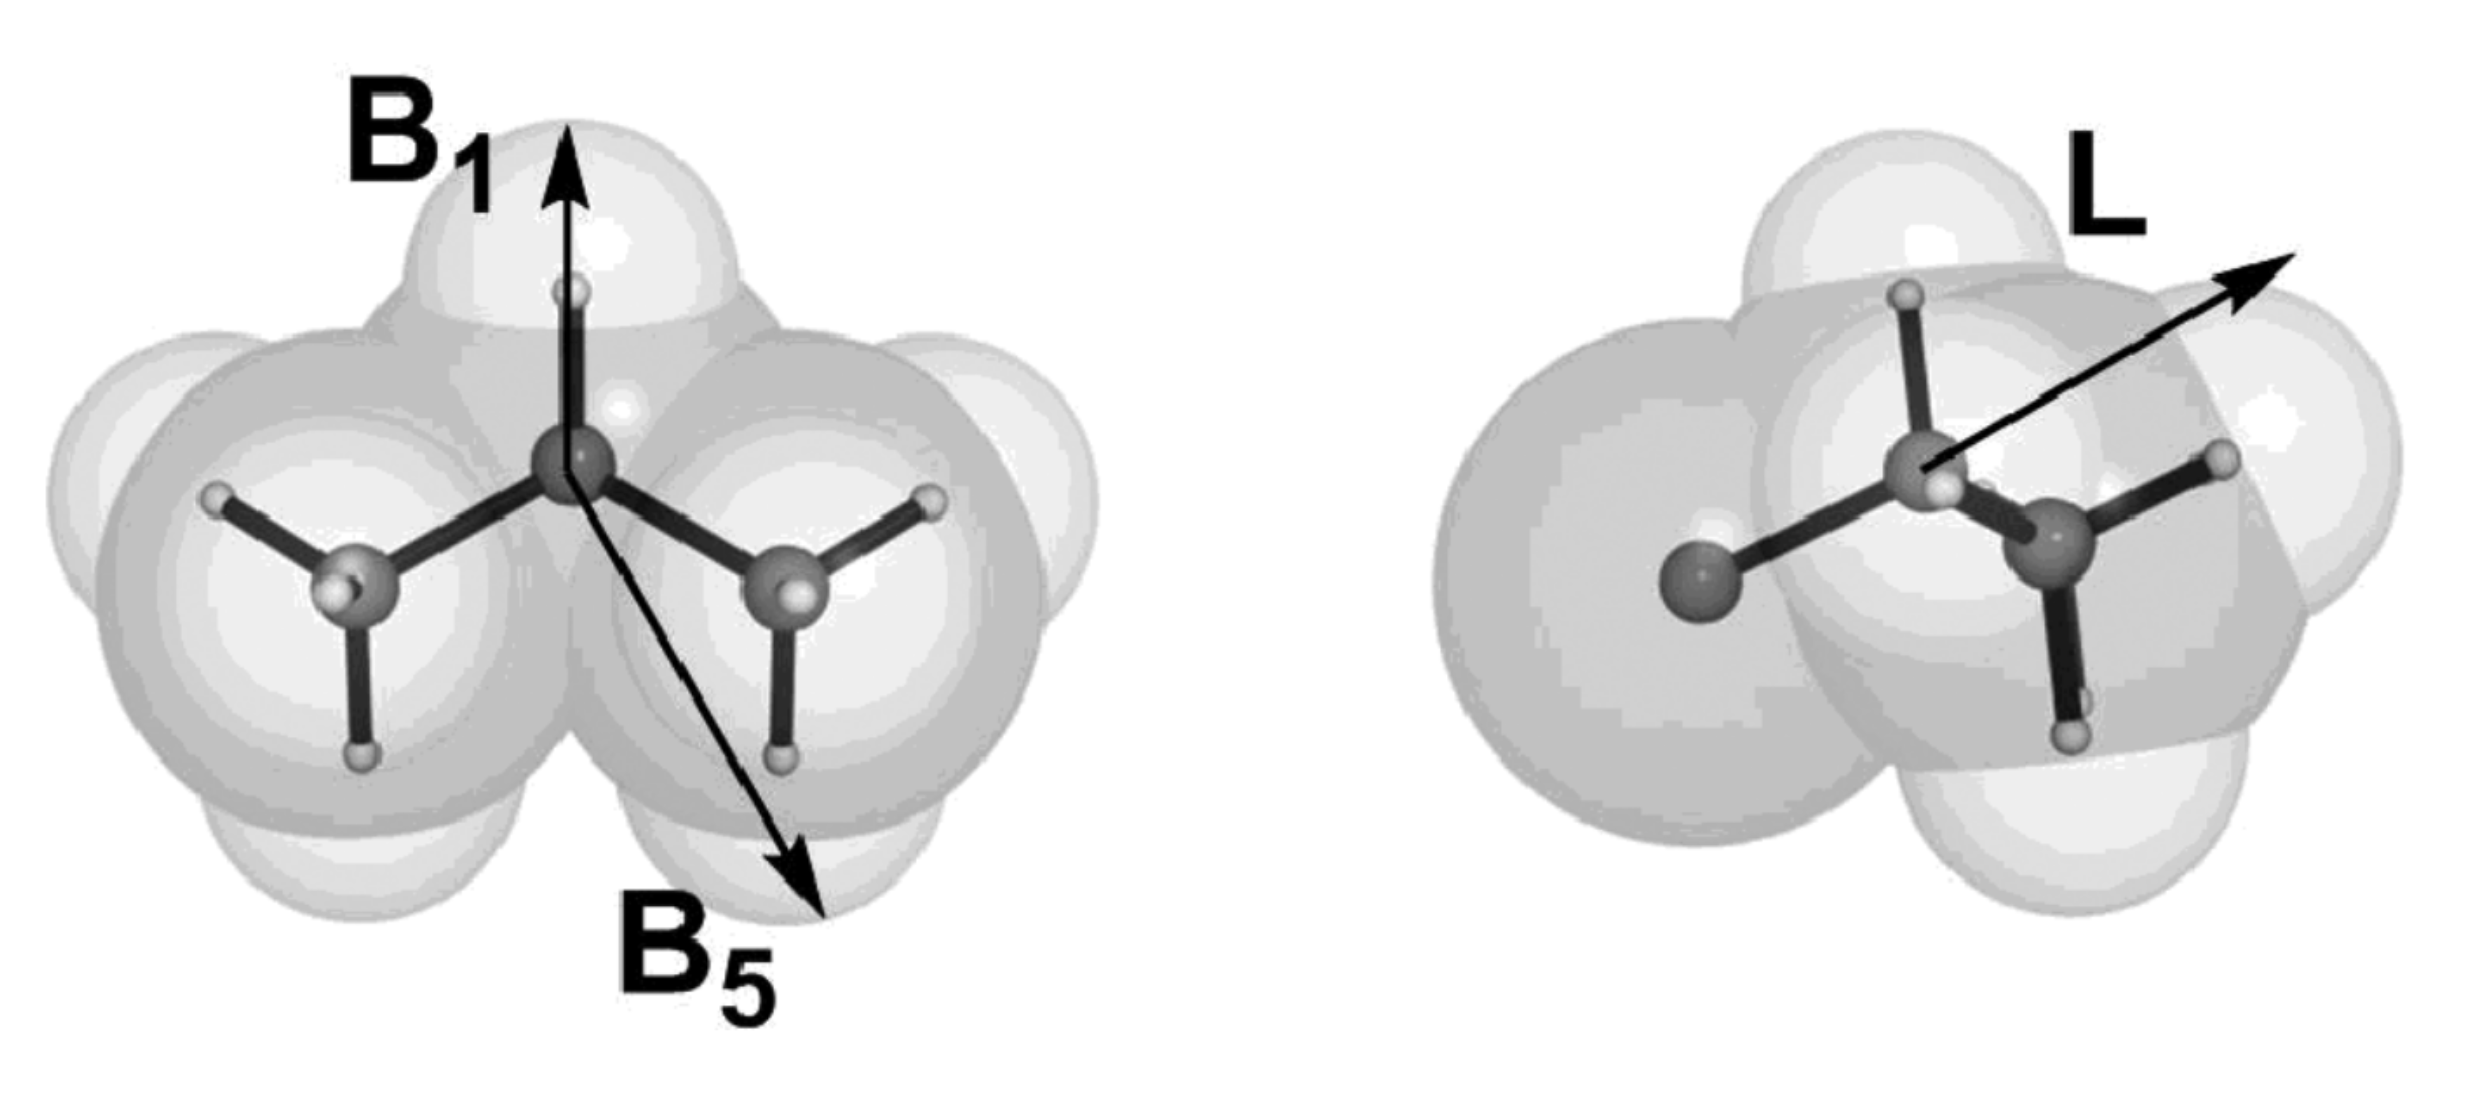
\includegraphics[width=0.75\linewidth]{figures/CH4-sterimol.png}
  \caption{Sterimol parameters. The parameter $L$ describes extension along this axis, while $B_1$ and $B_5$ describe the minimum and maximum widths perpendicular to it.}
  \label{fig4-3:sterimol}
\end{figure}

\solution{4cm}{%
  \textbf{A useful descriptor should be:}
  \begin{itemize}
    \item invariant;
    \item discriminating;
    \item chemically relevant;
    \item no more complex than required.
  \end{itemize}
}

\section{Comparing molecules}

Once molecules have been represented using a common set of descriptors, their similarity can be expressed quantitatively.
The simplest approach is to treat each descriptor as an axis and compare the positions of two molecules in the resulting descriptor space. For continuous descriptors, a common measure is the \keypoint{Euclidean distance} between two descriptor vectors.

\solution{6.5cm}{%
  \centering

  molecule \textbf{A} $\longrightarrow \mathbf{x}_{\mathrm{A}}$
  \qquad
  molecule \textbf{B} $\longrightarrow \mathbf{x}_{\mathrm{B}}$

  \vspace{0.9em}

  molecular comparison
  $\longrightarrow$
  distance between $\mathbf{x}_{\mathrm{A}}$ and $\mathbf{x}_{\mathrm{B}}$
  
    \vspace{0.9em}

  \begin{equation}
    d_{\mathrm{AB}}
    =
    \left[
      \sum_{j=1}^{p}
      \left(x_{\mathrm{A}j}-x_{\mathrm{B}j}\right)^2
    \right]^{1/2}.
  \end{equation}
}

\subsection{Descriptor scaling}

Descriptor values can have very different numerical ranges and physical units.
For example, molecular mass may vary by hundreds of daltons, while an orbital energy may vary by only a few electronvolts and a buried-volume descriptor may be expressed as a percentage.
Without scaling, descriptors with the largest numerical variation can dominate a distance calculation.

A common transformation is therefore to centre and scale each descriptor,

  \begin{equation}
    z_{ij}
    =
    \frac{x_{ij}-\bar{x}_j}{s_j},
  \end{equation}

where $\bar{x}_j$ and $s_j$ are the mean and standard deviation of descriptor $j$ within the dataset.
After standardisation, each descriptor is expressed relative to its variation within that dataset rather than in its original physical units.
Hence, all descriptors contribute comparably to the final distance.

\subsection{Similarity between fingerprints}

The molecular fingerprints introduced previously are binary representations rather than collections of continuous physicochemical descriptors.
For binary fingerprints, similarity is commonly measured using the \keypoint{Tanimoto coefficient}.\mcite{Bajusz2015}
If fingerprint \textbf{A} contains $a$ active bits, fingerprint \textbf{B} contains $b$ active bits, and $c$ bits are active in both fingerprints, then

\solution{3.0cm}{%
  \begin{equation}
    T_{\mathrm{AB}}
    =
    \frac{c}{a+b-c}.
  \end{equation}
}

The Tanimoto coefficient ranges from zero for fingerprints with no shared active bits to one for identical fingerprints.
It therefore measures similarity according to the structural features encoded by that particular fingerprint.

For a collection of molecules, similarities can be calculated between every unique pair of fingerprints.
For $N$ molecules, the number of pairwise comparisons is

  \begin{equation}
    N_{\mathrm{pairs}}
    =
    \frac{N(N-1)}{2}.
  \end{equation}

For example, a collection of 100 molecules contains 4950 unique molecular pairs.
The complete set of pairwise similarities can be arranged as a symmetric similarity matrix,

  \begin{equation}
    \mathbf{T}
    =
    \begin{bmatrix}
      1 & T_{12} & T_{13} & \cdots & T_{1N} \\
      T_{21} & 1 & T_{23} & \cdots & T_{2N} \\
      T_{31} & T_{32} & 1 & \cdots & T_{3N} \\
      \vdots & \vdots & \vdots & \ddots & \vdots \\
      T_{N1} & T_{N2} & T_{N3} & \cdots & 1
    \end{bmatrix}.
  \end{equation}

The matrix is symmetric because $T_{ij}=T_{ji}$, and every diagonal element is one because each molecule is identical to itself.
If the objective is only to find molecules similar to one query structure, the query fingerprint instead needs to be compared only with the other molecules in the collection.

\begin{conceptbox}
  \keypoint{Molecular similarity is representation dependent.} Euclidean distance compares molecules according to continuous descriptors, while the Tanimoto coefficient compares the features encoded in a molecular fingerprint.
  Two molecules can appear similar in one representation and not in another.
\end{conceptbox}

\solution{3.6cm}{%
  \centering

  \textbf{molecular similarity}
  $=$ \\[0.4em]
  \textbf{representation} \\[0.4em]
  $+$ 
  \textbf{preprocessing} \\[0.4em]
  $+$ 
  \textbf{comparison metric}
}

Once a common representation and metric have been chosen, the collection of molecular positions defines a \keypoint{chemical space} that can be explored for similarities, differences, gaps, and regions of interest.

\section{Mapping chemical spaces}

Chemical space becomes most useful when its axes correspond to chemically meaningful properties.
Ligand design provides an early example because both electronic donation and steric demand can influence the behaviour of a metal catalyst.
Tolman's work on monodentate phosphorus ligands provides a particularly useful historical example.\mcite{Tolman1977}
Electronic effects can be described using the Tolman electronic parameter, while steric demand can be described using the Tolman cone angle.
Plotting the two parameters against one another converts a list of ligand properties into a two-dimensional ligand space (Fig.~\ref{fig4-4:tolman-ligand-space})
A ligand-selection problem can therefore be reframed from choosing familiar structures to choosing molecules that sample distinct regions of property space.

\begin{figure}[htbp]
  \centering
  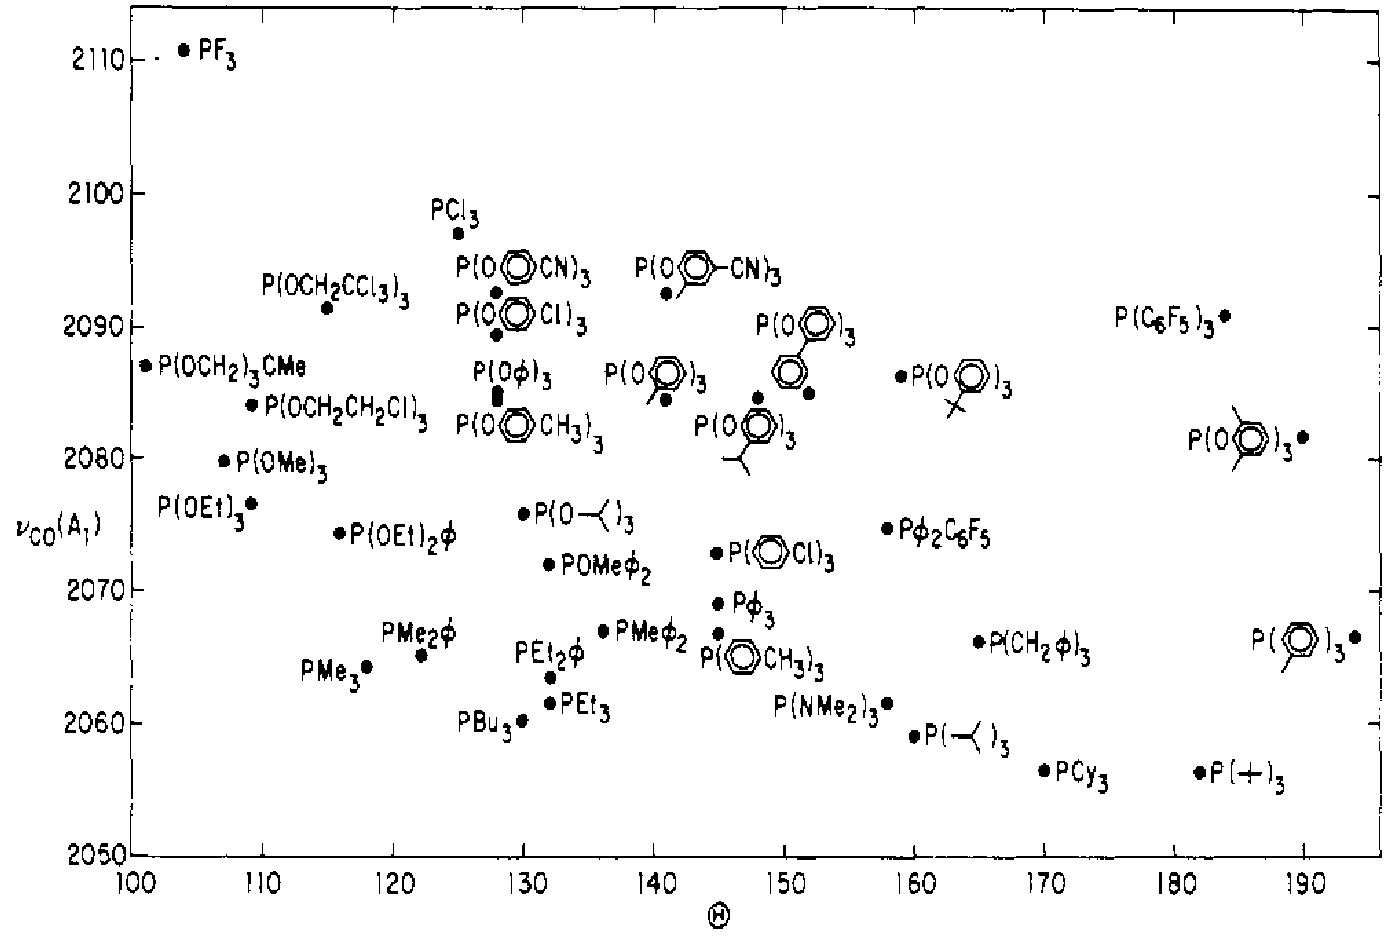
\includegraphics[width=0.82\linewidth]{figures/CH4-tolman.png}
  \caption{
    Steric--electronic ligand space constructed using Tolman's electronic and steric parameters.
    Ligands close together on the map have similar values for the two selected properties, while distant ligands differ more strongly in steric demand, electronic character, or both.
  }
  \label{fig4-4:tolman-ligand-space}
\end{figure}

There is no requirement for a chemical space to use electronic and steric axes.
The descriptors should instead reflect the molecular variation relevant to the problem being investigated.
A shape-based space, for example, may organise molecules according to their three-dimensional geometry (Fig.~\ref{fig4-5:pmi-shape-space}).\mcite{Firth2012}

\begin{figure}[htbp]
  \centering
  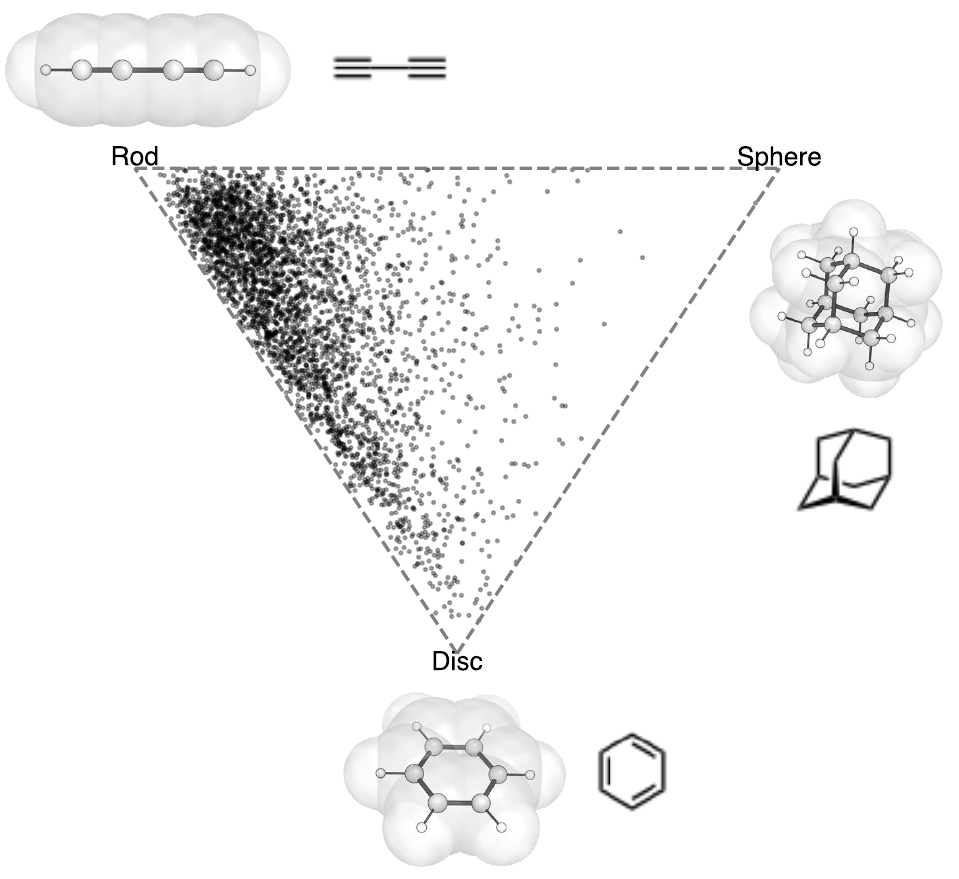
\includegraphics[width=0.72\linewidth]{figures/CH4-pmi.png}
  \caption{
    Schematic molecular shape space based on principal moments of inertia.
    The same idea of molecular distance can be applied to geometrical rather than steric--electronic descriptors.
  }
  \label{fig4-5:pmi-shape-space}
\end{figure}

The Tolman and shape-space examples describe different molecular questions and therefore arrange molecules differently.
This is an important feature rather than a failure of chemical-space analysis: the representation determines which molecular relationships are emphasised.

Two-dimensional maps are easy to inspect because both descriptor axes can be drawn directly.
Modern ligand libraries contain many steric, electronic, geometric, and whole-molecule descriptors, so the corresponding ligand space \keypoint{multidimensional}.
For example, \textit{kraken} combines large numbers of calculated descriptors for organophosphorus ligands rather than relying on one steric and one electronic coordinate.
Every descriptor adds another axis and every ligand remains a point defined by its descriptor values.
The practical problem is that a space containing many descriptor axes can no longer be visualised directly.
This motivates \keypoint{dimensionality reduction}: constructing a lower-dimensional view that retains useful structure from the original descriptor space.

\section{Dimensionality reduction}

Tolman's ligand map can be drawn directly because it contains only two descriptor axes.
Modern descriptor libraries contain many steric, electronic, and geometric, so the corresponding chemical space cannot be inspected directly.
\keypoint{Dimensionality reduction} constructs a lower-dimensional representation that preserves selected structure from the original descriptor space.
The resulting axes need not correspond to individual molecular descriptors, and information is generally lost when a high-dimensional space is projected into only two or three dimensions.

\subsection{Principal component analysis}

\keypoint{Principal component analysis (PCA)} constructs new orthogonal axes, called principal components, from linear combinations of the original descriptors.\mcite{Pearson1901}
The first principal component is chosen to capture the greatest possible variance in the dataset.
The second captures the greatest remaining variance while being orthogonal to the first, and subsequent components follow the same principle.

Each principal component is a weighted combination of the original descriptors,

\begin{equation}
  \mathrm{PC}_k
  =
  w_{k1}x_1
  + w_{k2}x_2
  + \cdots
  + w_{kp}x_p.
\end{equation}

The coefficients $w_{kj}$ describe how strongly descriptor $j$ contributes to principal component $k$.
PCA therefore rotates the original descriptor coordinate system to obtain new axes that summarise the major directions of variation in the dataset.

\solution{8cm}{
% \begin{figure}[htbp]
  \centering
  \resizebox{\linewidth}{!}{%
    \begin{tikzpicture}[
        transform shape,
        axis/.style={draw=darkGrey,line width=1.5pt,->,>=Stealth},
        datum/.style={fill=darkBlue,draw=darkBlue},
        pc/.style={draw=darkRed,line width=2.5pt,->,>=Stealth},
        bad/.style={draw=darkGreen,line width=2.5pt,->,>=Stealth},
        project/.style={draw=darkGrey,dashed,line width=1.0pt},
        spread/.style={draw=darkGrey,line width=1.5pt,<->,>=Stealth},
        label/.style={font=\small\sffamily,text=darkGrey,align=center},
        title/.style={font=\sffamily,text=darkGrey,align=center}
      ]

      \path[use as bounding box] (0,-0.5) rectangle (17.3,6.7);

      % Original 2D descriptor space
      \node[title] at (4.1,6.25) {Original descriptor space};
      \draw[axis] (0.8,0.9) -- (7.8,0.9);
      \draw[axis] (0.8,0.9) -- (0.8,5.7);
      \node[label,anchor=east] at (7.65,0.43) {$x_1$};
      \node[label,rotate=90] at (0.28,4.85) {$x_2$};

      % Elongated correlated cloud
      \foreach \x/\y in {
        1.55/1.50,1.95/1.72,2.35/1.82,2.65/2.13,
        3.05/2.18,3.35/2.47,3.70/2.52,4.05/2.88,
        4.40/2.95,4.75/3.23,5.10/3.38,5.42/3.63,
        5.78/3.78,6.10/4.05,6.48/4.13,6.80/4.48,
        2.55/1.75,3.85/2.95,5.25/3.08,6.15/4.42
      } {
        \fill[datum] (\x,\y) circle (3.3pt);
      }

      % Directions through the cloud
      \draw[pc] (2.0,1.50) -- (6.75,4.70);
      \node[label,text=darkRed,anchor=west] at (6.78,4.72)
        {large variance};

      \draw[bad] (3.00,4.20) -- (5.20,1.25);
      \node[label,text=darkGreen,anchor=west] at (1.28,4.65)
        {small variance};

      % Arrow to one-dimensional projections
      \draw[axis] (8.25,3.25) -- (9.15,3.25);

      % Good projection
      \node[title] at (13.20,6.25) {Projected onto one axis};
      \draw[axis] (9.65,4.55) -- (16.55,4.55);
      \foreach \x in {10.00,10.30,10.68,11.05,11.45,11.85,12.25,12.72,13.15,13.60,14.05,14.48,14.90,15.28,15.70,16.00} {
        \fill[datum] (\x,4.55) circle (3.3pt);
      }
      \draw[spread] (10.00,5.15) -- (16.00,5.15);
      \node[label,text=darkRed] at (13.00,5.55)
        {projection retains broad variation};

      % Poor projection
      \draw[axis] (9.65,1.70) -- (16.55,1.70);
      \foreach \x in {12.10,12.26,12.37,12.49,12.62,12.72,12.84,12.96,13.08,13.20,13.31,13.43,13.54,13.66,13.78,13.91} {
        \fill[datum] (\x,1.70) circle (3.3pt);
      }
      \draw[spread] (12.10,2.30) -- (13.91,2.30);
      \node[label,text=darkGreen] at (13.00,2.70)
        {projection collapses variation};

      \node[label] at (13.00,0.82)
        {PCA selects directions that maximise retained variance};

    \end{tikzpicture}%
  }
%   \caption{
%     Dimensionality reduction depends on the direction of projection.
%     Projecting the same descriptor data along different directions preserves different amounts of variation.
%     Principal component analysis selects orthogonal directions that retain the greatest variance in the dataset.
%   }
%   \label{fig4-6:pca-projection}
% \end{figure}
  \vspace{2em}
  \textbf{original axes}
  $=$
  molecular descriptors

  \textbf{new PCA axes}
  $=$
  orthogonal descriptors explaining most variance

}

After PCA, each molecule has a coordinate along each principal component.
These coordinates are the \keypoint{scores}, and plotting the scores of the first two principal components produces the familiar PCA map.
The descriptor coefficients used to construct each principal component are the \keypoint{loadings}.
Loadings allow the new axes to be interpreted in terms of the original molecular descriptors and are therefore essential when a chemical interpretation of a PCA map is required.

\begin{figure}[htbp]
  \centering

  \resizebox{\linewidth}{!}{%
    \begin{tikzpicture}[
        transform shape,
        axis/.style={draw=darkGrey,line width=1.5pt,->,>=Stealth},
        datum/.style={fill=darkBlue,draw=darkBlue},
        loading/.style={draw=darkRed,line width=2.3pt,->,>=Stealth},
        loadingtwo/.style={draw=darkGreen,line width=2.3pt,->,>=Stealth},
        guide/.style={draw=darkGrey,dashed,line width=1.0pt},
        label/.style={font=\small\sffamily,text=darkGrey,align=center},
        title/.style={font=\sffamily,text=darkGrey,align=center}
      ]

      \path[use as bounding box] (0,-0.5) rectangle (17.3,6.8);

      % Scores plot
      \node[title] at (4.15,6.30) {Scores: where are the molecules?};
      \draw[axis] (0.8,3.20) -- (7.75,3.20);
      \draw[axis] (4.15,0.75) -- (4.15,5.90);
      \node[label,anchor=east] at (7.60,2.73) {PC1};
      \node[label,rotate=90] at (3.58,5.10) {PC2};

      \foreach \x/\y in {
        1.55/2.10,2.05/2.55,2.45/1.72,2.82/2.88,
        3.35/3.52,3.65/4.15,4.05/3.82,
        4.60/3.42,5.05/4.20,5.35/3.72,
        5.92/2.55,6.35/2.02,6.78/2.82
      } {
        \fill[datum] (\x,\y) circle (3.6pt);
      }

      \node[label,anchor=west] at (2.15,0)
        {each point = one molecule};

      % Divider arrow
      \draw[axis] (8.20,3.20) -- (9.05,3.20);

      % Loading plot
      \node[title] at (13.05,6.30) {Loadings: what defines the axes?};
      \draw[axis] (9.65,3.20) -- (16.55,3.20);
      \draw[axis] (13.05,0.75) -- (13.05,5.90);
      \node[label,anchor=east] at (16.40,2.73) {PC1};
      \node[label,rotate=90] at (12.48,5.10) {PC2};

      % Descriptor loading vectors
      \draw[loading] (13.05,3.20) -- (15.72,4.72);
      \node[label,text=darkRed,anchor=west] at (15.80,4.76)
        {$x_1$: steric};

      \draw[loading] (13.05,3.20) -- (15.45,2.02);
      \node[label,text=darkRed,anchor=west] at (15.52,1.98)
        {$x_2$: size};

      \draw[loadingtwo] (13.05,3.20) -- (11.15,5.00);
      \node[label,text=darkGreen,anchor=east] at (11.05,5.05)
        {$x_3$: electronic};

      \draw[loadingtwo] (13.05,3.20) -- (10.60,2.15);
      \node[label,text=darkGreen,anchor=east] at (10.50,2.10)
        {$x_4$: polarity};

      \node[label] at (13.05,0)
        {arrows describe descriptor contributions};

    \end{tikzpicture}%
  }

  \caption{
    Relationship between PCA scores and loadings.
    Scores describe the positions of molecules in principal-component space.
    Loadings describe how the original descriptors contribute to each principal component and  provide a route to chemical interpretation of the new axes.
  }
  \label{fig4:pca-scores-loadings}
\end{figure}

\solution{3cm}{%
  \centering

  \textbf{scores}
  $\longrightarrow$
  where are the molecules?

  \vspace{0.8em}

  \textbf{loadings}
  $\longrightarrow$
  which descriptors define those directions?
}

\subsection{Explained variance}

Reducing dimensionality necessarily discards some information.
The \keypoint{explained variance} of a principal component reports how much of the total variation in the original dataset is represented along that component.
The cumulative explained variance of the retained components therefore provides one measure of how much information is preserved in a lower-dimensional map.

A two-dimensional PCA plot may be visually convenient while representing only part of the variation in the original descriptor space.
The percentage of variance explained by the displayed components should therefore be reported and considered when interpreting apparent distances, groups, or gaps.

\begin{conceptbox}
  \keypoint{A PCA map is a projection, not the chemical space itself.}
  Apparent molecular relationships in a two-dimensional scores plot are useful only to the extent that the retained components capture the variation relevant to the chemical question.
  Loadings and explained variance are therefore part of the interpretation, not optional statistical details.
\end{conceptbox}

\subsection{Nonlinear maps}

Other dimensionality-reduction methods, including t-SNE and UMAP, can produce useful low-dimensional maps when relationships in the original descriptor space are not well represented by linear projections.
These methods are particularly useful for visualising local neighbourhoods and complex high-dimensional structure, but their map axes do not have the direct descriptor-based interpretation of PCA loadings.
The geometry of a nonlinear map can also depend strongly on the method and its settings.
Distances and cluster separation in a two-dimensional visualisation should not automatically be interpreted as distances in the original descriptor space.

\section{Mapping chemical spaces}

\subsection{Ligand Knowledge Bases (LKB)}

Tolman's map shows how two chemically meaningful parameters can organise ligands into a useful property space.
Modern ligand datasets extend the same idea by combining many calculated steric, electronic, and geometric descriptors.
Dimensionality reduction then provides a way to visualise the dominant patterns within this higher-dimensional space.

\begin{figure}[htbp]
  \centering
  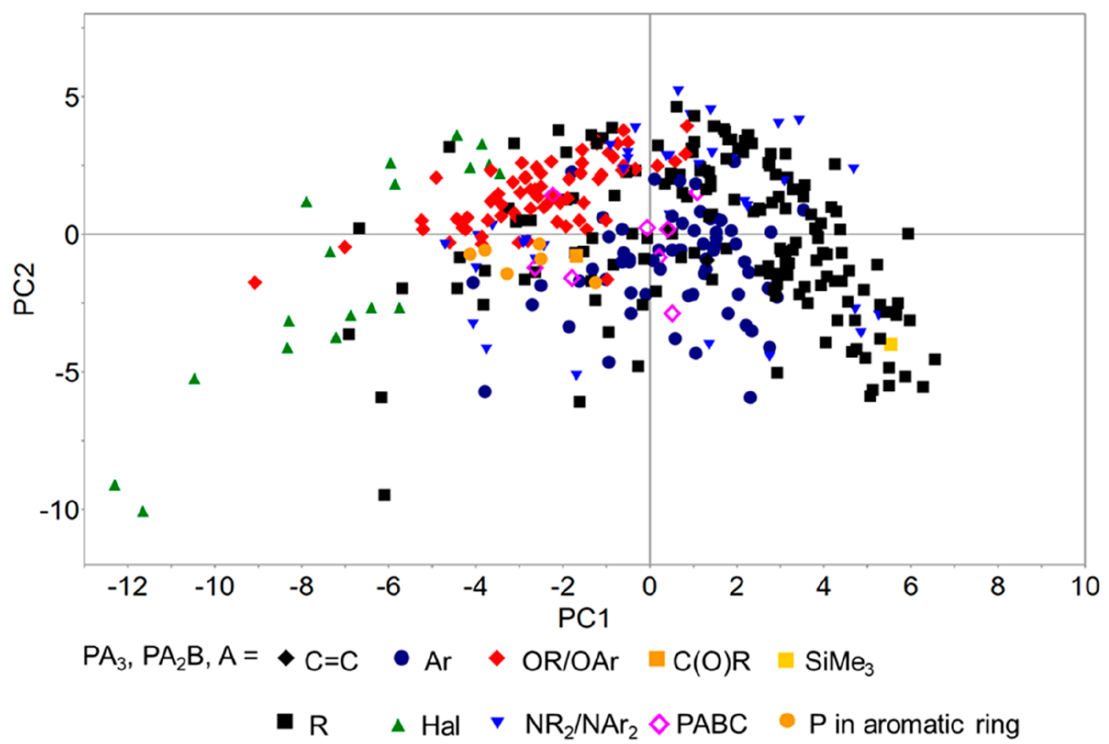
\includegraphics[width=0.88\linewidth]{figures/CH4-LKB-P.png}
  \caption{
    PCA map of phosphine ligand knowledge map. There are 28 descriptors calculated for 366 ligands; \textit{ca.} 62\% of variance is captured. 
  }
  \label{fig4-6:fey-lkb-p}
\end{figure}

Work by Fey and co-workers provides a useful modern continuation of the Tolman approach.\mcite{Durand2021}
Ligand knowledge bases collect steric and electronic descriptors for large sets of ligands and use principal component analysis to obtain lower-dimensional maps of ligand property space (Fig.~\ref{fig4-6:fey-lkb-p}).
A useful feature of this representation is that molecular structure is not used as the sole definition of similarity.
Ligands with different structural motifs may occupy similar regions when their calculated properties are similar, while apparently related ligands can separate when they differ strongly in the descriptors that define the map.
A diverse selection of ligands can be designed to span different regions of property space rather than simply collecting ligands with visibly different structures.

\begin{conceptbox}
If two candidate ligands occupy almost the same region of a chosen property space, testing both may provide  little additional coverage of that representation.
Selecting ligands from distinct regions can provide a broader survey of steric and electronic effects using a smaller experimental set.
\end{conceptbox}

\subsection{Exploring solvent space}

Solvents provide another intuitive example because solvent choice depends on several physical and chemical properties simultaneously.
A solvent can also be represented as a point in a multidimensional property space.

\solution{4cm}{%

Properties relevant to solvent comparison may include:
\begin{itemize}
  \item polarity
  \item boiling point
  \item environmental safety
  \item $\cdots$
\end{itemize}
}


The \keypoint{ACS Green Chemistry Institute Pharmaceutical Roundtable} is an interactive solvent tool based on principal component analysis of 70 solvent properties.\mcite{Alder2016}
The tool uses a PCA map to organise solvents according to their physical and chemical similarity and supplements this map with information including functional groups, physical properties, and environmental data.
The map provides a practical way to search for alternatives to a familiar solvent (Fig.~\ref{fig4-7:acs-solvent-replacement}).

\begin{figure}[htbp]
  \centering
  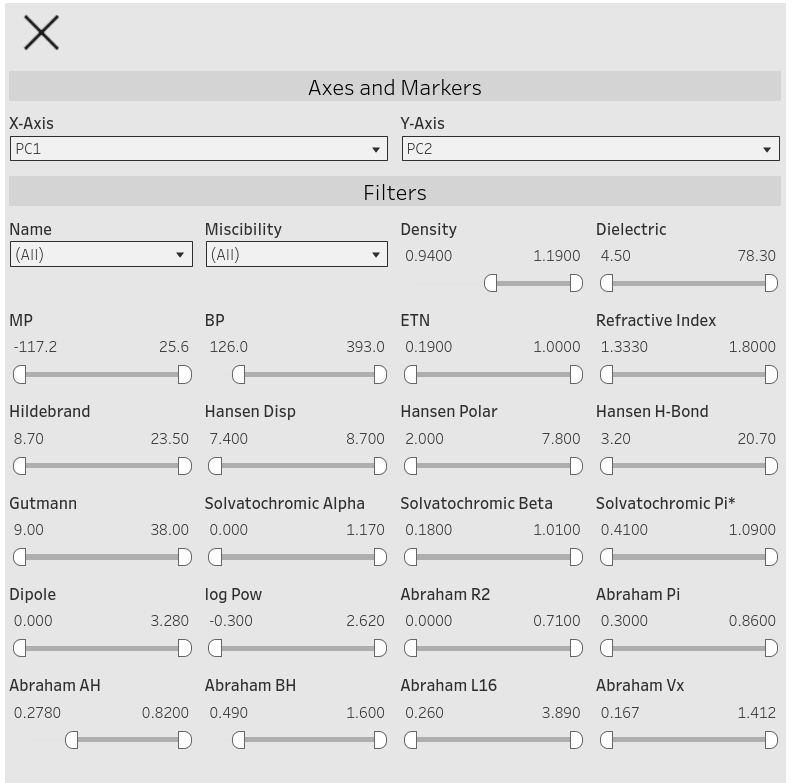
\includegraphics[width=0.45\linewidth]{figures/CH4-ACS-settings.png}
  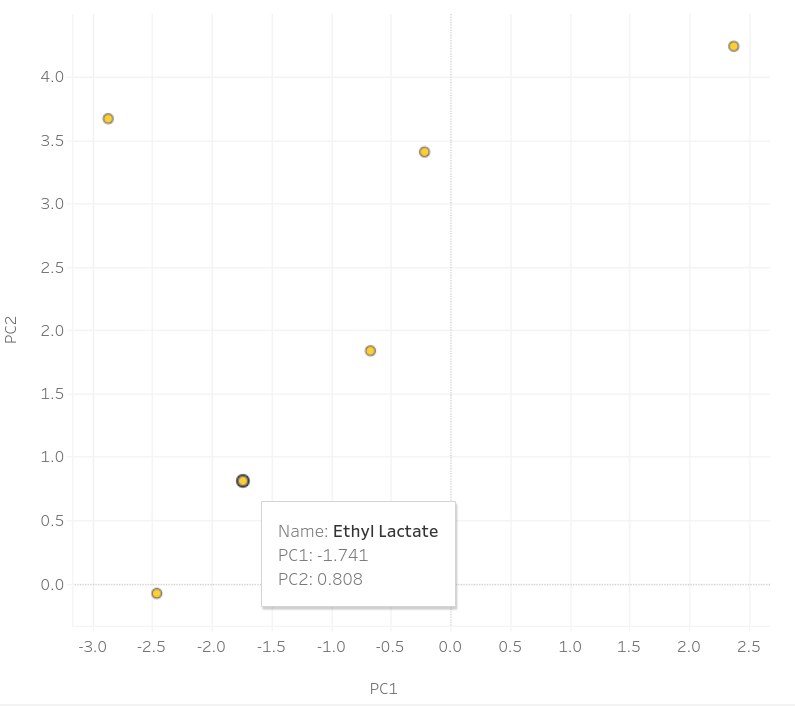
\includegraphics[width=0.45\linewidth]{figures/CH4-ACS-results.png}
  \caption{
    Example use of the ACS Solvent Tool to identify candidate replacements for a solvent.
  }
  \label{fig4-7:acs-solvent-replacement}
\end{figure}

\section{Clustering and representative selection}

Chemical-space maps can reveal densely populated regions, isolated molecules, and gaps in the sampled space.
When the number of possible molecules is much larger than the number of experiments that can be performed, these patterns can be used to select a smaller and more informative subset.
\keypoint{Clustering} groups molecules according to their proximity in a chosen representation.
Unlike the regression and classification problems introduced earlier, clustering does not require a target property: the groups are identified from the molecular representation itself.

\begin{conceptbox}
  \keypoint{Clusters are properties of a representation, not intrinsic labels carried by molecules.}
  Changing the descriptors or the way distances are calculated can change which molecules are grouped together.
\end{conceptbox}

\solution{8.0cm}{%
  \centering

  \resizebox{\linewidth}{!}{%
    \begin{tikzpicture}[
        transform shape,
        axis/.style={draw=darkGrey,line width=1.4pt,->,>=Stealth},
        arrow/.style={draw=darkGrey,line width=2.0pt,->,>=Stealth},
        bluepoint/.style={fill=darkBlue,draw=darkBlue},
        redpoint/.style={fill=darkRed,draw=darkRed},
        greenpoint/.style={fill=darkGreen,draw=darkGreen},
        greyPoint/.style={fill=darkGrey,draw=darkGrey},
        centroid/.style={fill=white,draw=darkGrey,line width=1.6pt},
        representative/.style={fill=darkYellow,draw=darkGrey,line width=1.1pt},
        clusterblue/.style={fill=paleBlue,draw=darkBlue,line width=1.5pt,opacity=0.55},
        clusterred/.style={fill=paleRed,draw=darkRed,line width=1.5pt,opacity=0.55},
        clustergreen/.style={fill=paleGreen,draw=darkGreen,line width=1.5pt,opacity=0.55},
        label/.style={font=\small\sffamily,text=darkGrey,align=center},
        title/.style={font=\sffamily,text=darkGrey,align=center}
      ]

      \path[use as bounding box] (0,-0.55) rectangle (17.3,7.3);

      % ---------------------------------------------------------------------
      % Panel 1: chemical space
      % ---------------------------------------------------------------------
      \node[title] at (2.6,6.80) {Chemical space};
      \draw[axis] (0.55,1.15) -- (4.65,1.15);
      \draw[axis] (0.55,1.15) -- (0.55,6.15);
      \node[label,anchor=east] at (4.55,0.72) {PC1};
      \node[label,rotate=90] at (0.12,5.40) {PC2};

      % Three latent groups, initially all shown identically.
      \foreach \x/\y in {
        1.00/2.10,1.28/2.36,1.55/2.02,1.72/2.55,1.95/2.28,
        2.52/4.55,2.78/4.85,3.02/4.48,3.18/5.10,3.42/4.72,
        3.02/2.25,3.30/2.45,3.56/2.13,3.78/2.67,4.05/2.37
      } {
        \fill[greyPoint] (\x,\y) circle (3.0pt);
      }

      % Arrow
      \draw[arrow] (4.95,3.65) -- (6.00,3.65);
      \node[label] at (5.47,4.10) {cluster};

      % ---------------------------------------------------------------------
      % Panel 2: clustered space
      % ---------------------------------------------------------------------
      \node[title] at (8.55,6.80) {Clusters};
      \draw[axis] (6.35,1.15) -- (10.75,1.15);
      \draw[axis] (6.35,1.15) -- (6.35,6.15);
      \node[label,anchor=east] at (10.65,0.72) {PC1};
      \node[label,rotate=90] at (5.92,5.40) {PC2};

      % Pale cluster regions first.
      \fill[clusterblue]
        plot[smooth cycle,tension=0.8] coordinates {
          (6.72,1.72) (7.45,1.62) (8.02,2.05) (7.88,2.87) (7.05,3.05) (6.62,2.48)
        };
      \fill[clusterred]
        plot[smooth cycle,tension=0.8] coordinates {
          (7.86,4.05) (8.35,3.86) (9.10,4.05) (9.46,4.90) (8.92,5.55) (8.08,5.40)
        };
      \fill[clustergreen]
        plot[smooth cycle,tension=0.8] coordinates {
          (8.68,1.72) (9.32,1.58) (10.20,1.95) (10.42,2.74) (9.78,3.18) (8.92,2.94)
        };

      \foreach \x/\y in {6.80/2.10,7.08/2.36,7.35/2.02,7.52/2.55,7.75/2.28}
        {\fill[bluepoint] (\x,\y) circle (3.0pt);}
      \foreach \x/\y in {8.02/4.55,8.28/4.85,8.52/4.48,8.68/5.10,8.92/4.72}
        {\fill[redpoint] (\x,\y) circle (3.0pt);}
      \foreach \x/\y in {9.02/2.25,9.30/2.45,9.56/2.13,9.78/2.67,10.05/2.37}
        {\fill[greenpoint] (\x,\y) circle (3.0pt);}

      % Centroids as open circles.
      \draw[centroid] (7.30,2.28) circle (6.0pt);
      \draw[centroid] (8.50,4.74) circle (6.0pt);
      \draw[centroid] (9.54,2.37) circle (6.0pt);

      % Arrow
      \draw[arrow] (11.05,3.65) -- (12.10,3.65);
      \node[label] at (11.58,4.10) {select};

      % ---------------------------------------------------------------------
      % Panel 3: representative molecules
      % ---------------------------------------------------------------------
      \node[title] at (14.75,6.80) {Representative molecules};
      \draw[axis] (12.45,1.15) -- (16.90,1.15);
      \draw[axis] (12.45,1.15) -- (12.45,6.15);
      \node[label,anchor=east] at (16.80,0.72) {PC1};
      \node[label,rotate=90] at (12.02,5.40) {PC2};

      % Original space faded into context.
      \foreach \x/\y in {
        12.90/2.10,13.18/2.36,13.45/2.02,13.62/2.55,13.85/2.28,
        14.12/4.55,14.38/4.85,14.62/4.48,14.78/5.10,15.02/4.72,
        15.12/2.25,15.40/2.45,15.66/2.13,15.88/2.67,16.15/2.37
      } {
        \fill[paleGrey] (\x,\y) circle (2.6pt);
      }

      % Selected nearest-to-centroid representatives.
      \fill[representative] (13.45,2.02) circle (5.2pt);
      \fill[representative] (14.62,4.48) circle (5.2pt);
      \fill[representative] (15.40,2.45) circle (5.2pt);

      \node[label,anchor=west] at (13.75,3.45)
        {one molecule selected\\from each region};

    \end{tikzpicture}%
  }
}

\subsection{Reaction scope as a selection problem}

Representative selection is also relevant when demonstrating the scope of a new synthetic method.
Substrate scopes are rarely unbiased samples of chemical space. 
A conventional substrate scope can be influenced by availability, familiarity, or the expectation that particular substrates will succeed.
\keypoint{Selection bias} arises because substrates are typically chosen based on availability, precedent, expected reactivity, or to demonstrate particular functional-group tolerance, while \keypoint{reporting bias} can arise when successful or informative reactions are preferentially reported over unsuccessful examples.
Systematic data-driven selection of diverse substrates provides one route towards constructing more representative tests of reaction generality.
Rana and co-workers developed a standardised substrate-selection strategy in which unsupervised learning is used to identify an unbiased substrate scope (Fig.~\ref{fig4:glorius-scope-1} and Fig.~\ref{fig4:glorius-scope-2}).\mcite{Rana2024}

\begin{figure}[htbp]
  \centering
  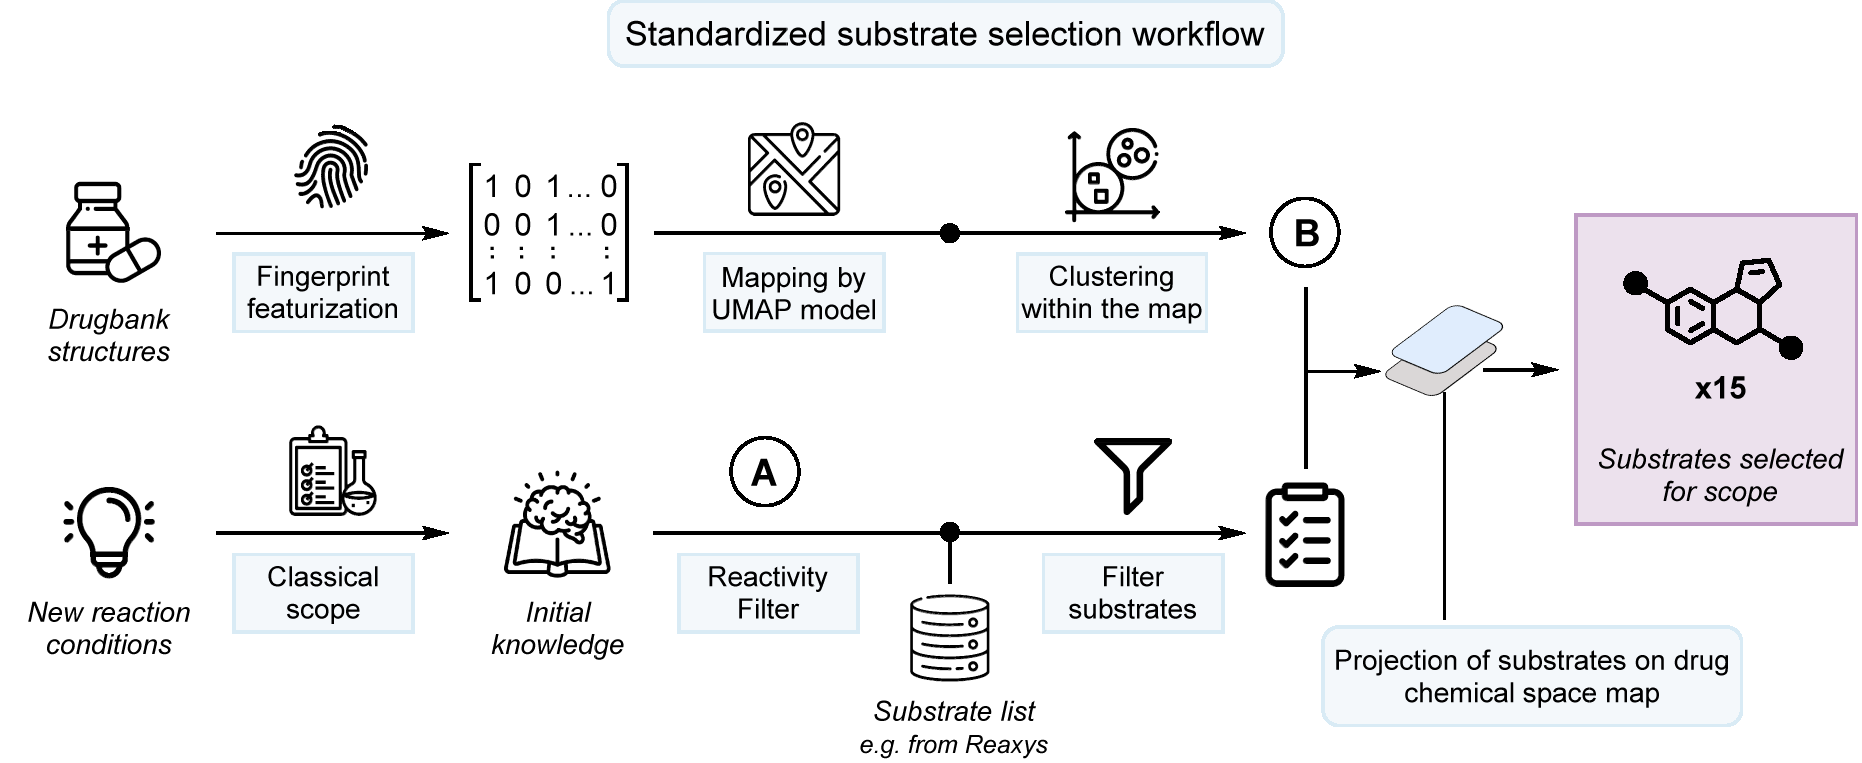
\includegraphics[width=\linewidth]{figures/CH4-glorius-1.png}
  \caption{
   Unbiased substrate scope selection strategy for evaluating reaction generality.
  }
  \label{fig4:glorius-scope-1}
\end{figure}

\begin{figure}[htbp]
  \centering
  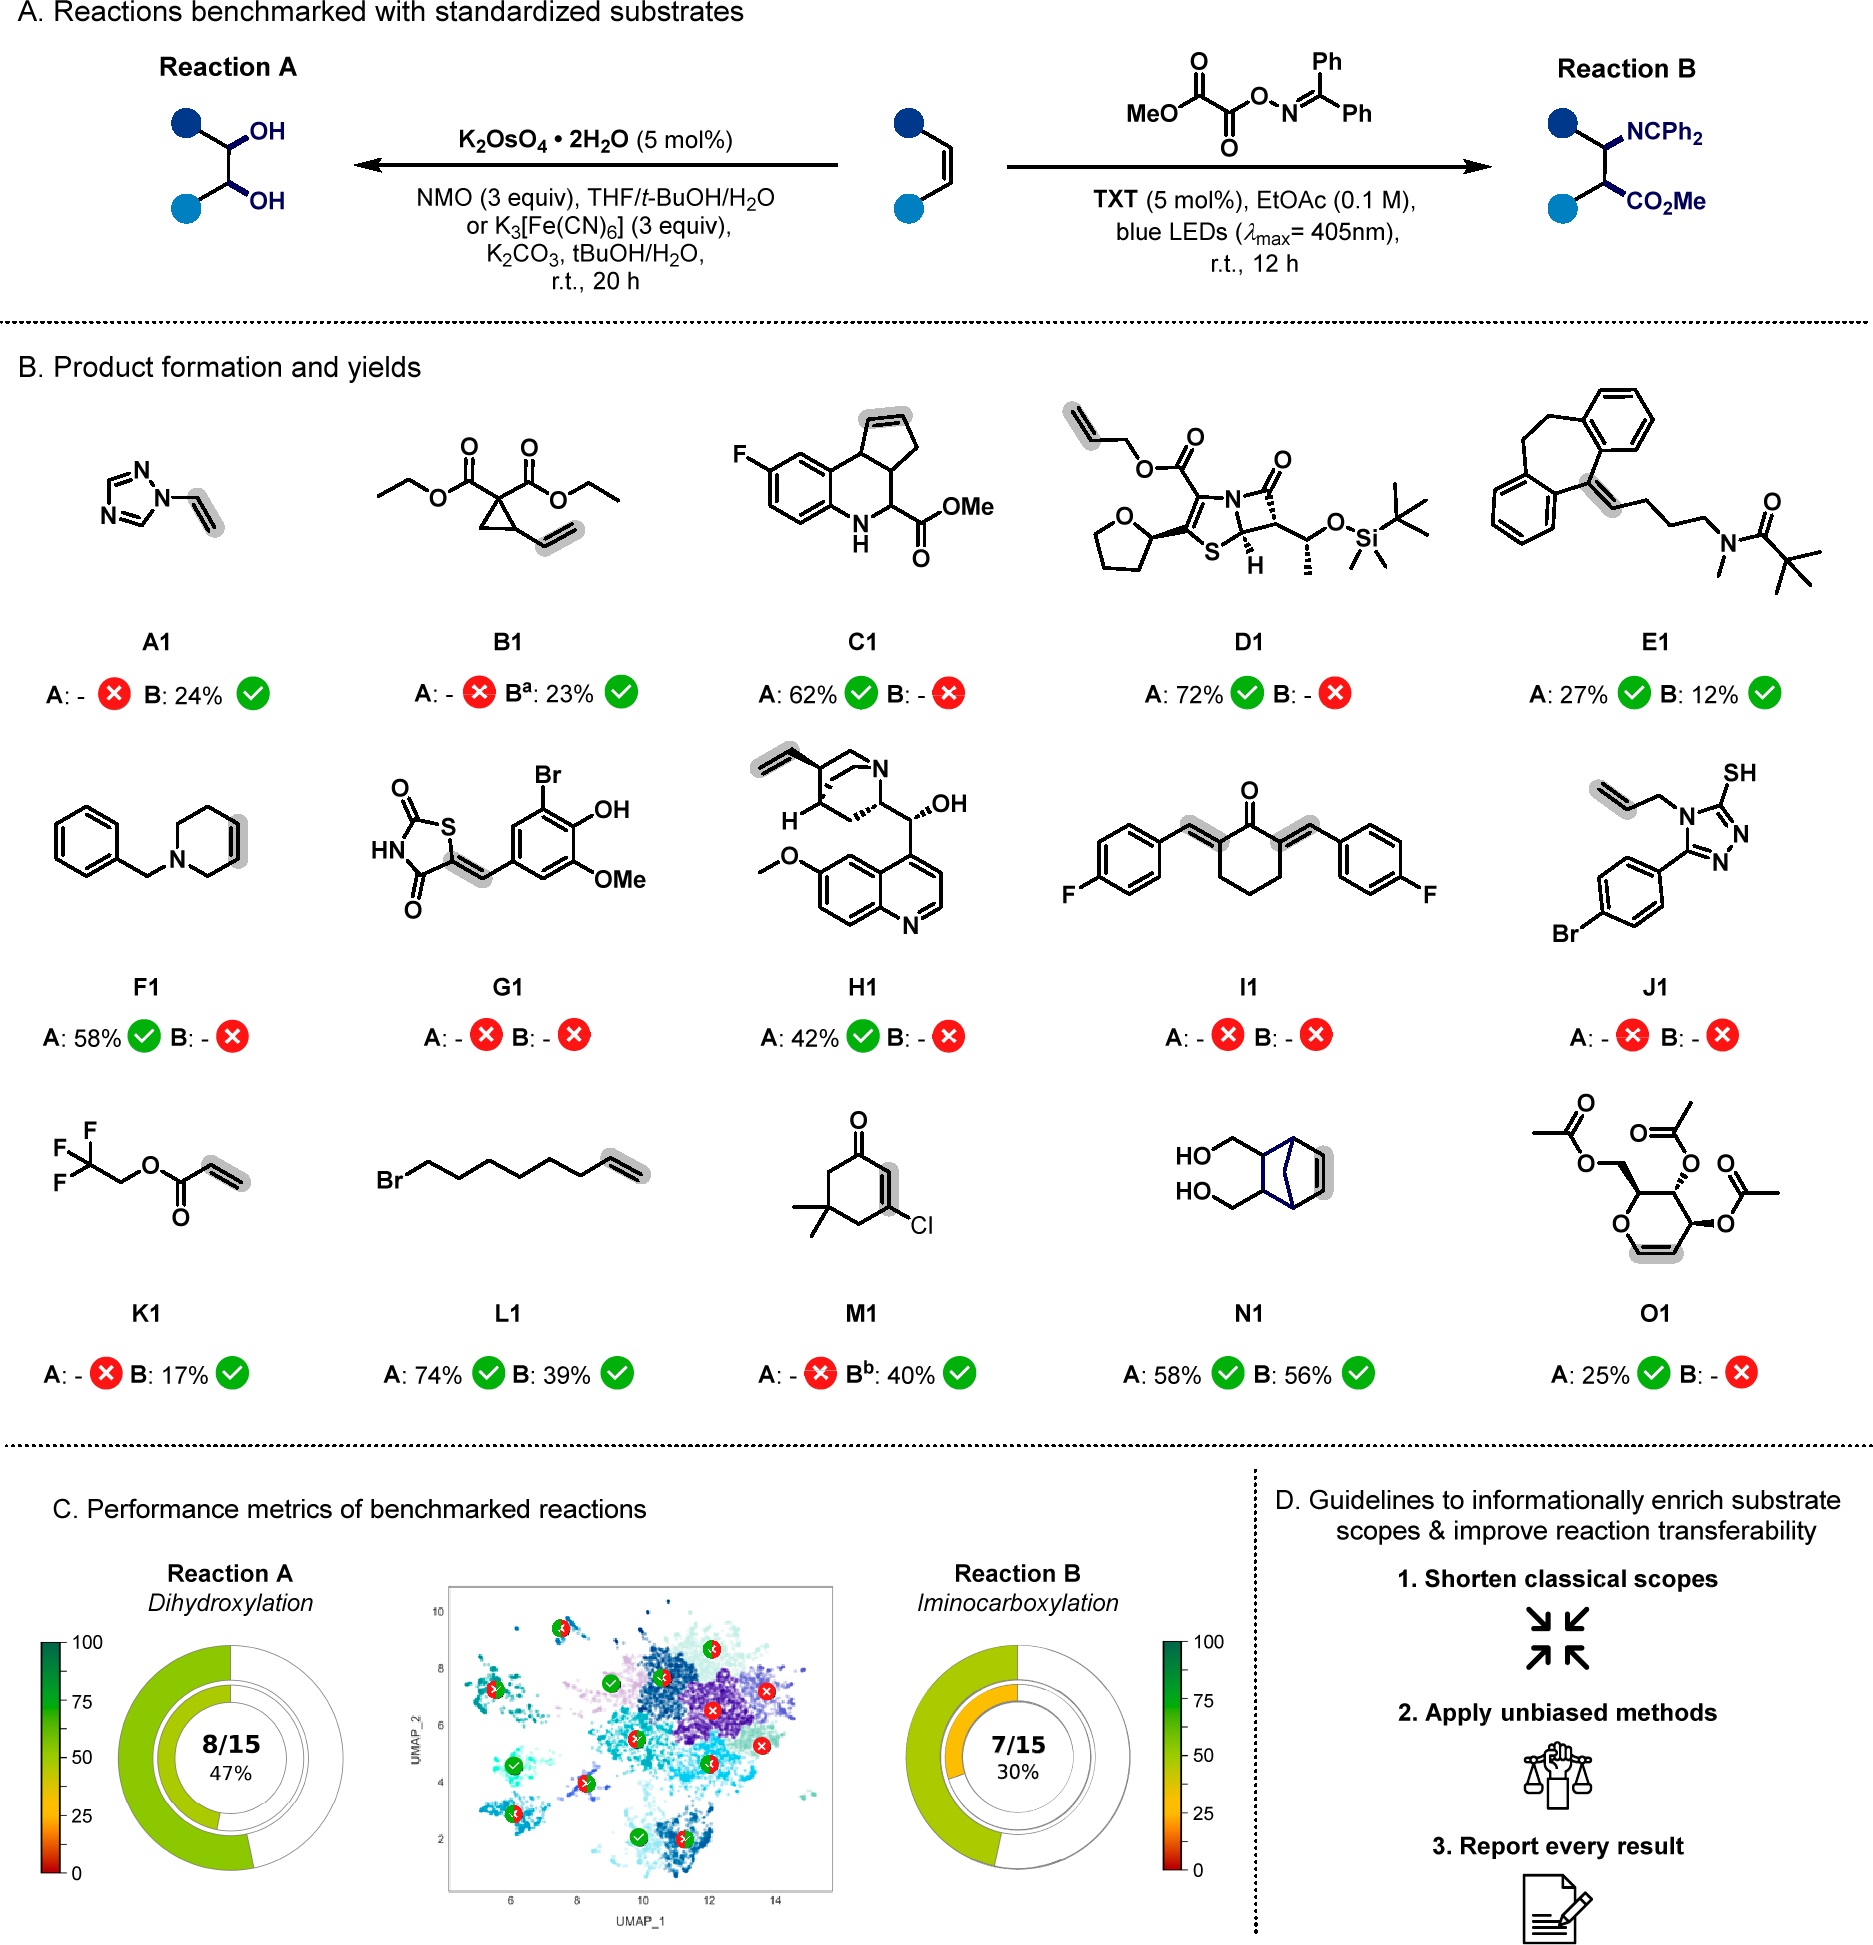
\includegraphics[width=\linewidth]{figures/CH4-glorius-2.png}
  \caption{
    Resulting generality assessment of two olefin functionalisation reactions.
  }
  \label{fig4:glorius-scope-2}
\end{figure}


\section{Summary}

Molecular descriptors convert selected aspects of chemical structure and properties into numerical representations.
Classical physical-organic parameters such as Hammett, Taft, and Tolman descriptors provide early examples of this idea, while modern descriptor libraries extend it to large collections of steric, electronic, geometric, and physicochemical properties.
Distances and similarities between these representations provide a quantitative definition of molecular neighbourhoods.
Dimensionality reduction allows high-dimensional molecular spaces to be visualised, while scores, loadings, and explained variance are required to interpret those projections critically.
Real ligand and solvent maps show how these methods can support chemical comparison and candidate selection.
Clustering and representative selection then turn a chemical-space map into an experimental-design tool.
The next chapter considers how descriptor-rich datasets can be converted into quantitative models of chemical reactivity and selectivity, and asks when such models provide chemical understanding rather than prediction alone.
